% !TEX encoding = UTF-8
% !TEX TS-program = pdflatex
% !TEX root = ../Tesi.tex
% !TEX spellcheck = en-EN

%************************************************
\chapter{Artificial Neural Network Training}
\label{cap:anntraining}
%************************************************

Fig. \ref{fig:019methodology} illustrates the methodology used. 
In the training phase (dashed lines)
$DEM$ simulations are performed
with random initial input parameters.
The behaviours obtained are used to train the
Artificial Neural Networks ($ANNs$) in a loop that continues until the
difference between the outputs of each $ANN$ and its simulations is below the
limit ($\Delta$) (see Section \ref{cap:ann}).
In the parameters identification phase (solid
lines) we identify valid input parameters by comparing (\textbf{=}) $ANNs$ and
experimental behaviours.

\begin{figure}[!htb] 
\centering 
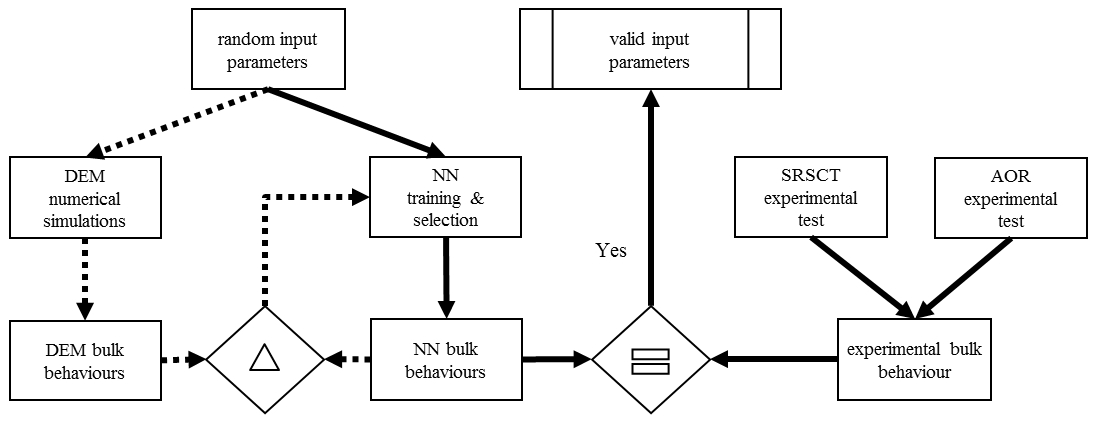
\includegraphics[width=.96\textwidth]{images/019methodology} 
\caption[Method]{Method. In the training phase (dashed lines)
$DEM$ simulations are performed
with random initial input parameters.
The behaviours obtained are used to train the
Artificial Neural Networks ($ANNs$) in a loop that continues until the
difference between the outputs of each $ANN$ and its simulations is below the
limit ($\Delta$).
In the parameters identification phase (solid
lines) we identify valid input parameters by comparing (\textbf{=}) $ANNs$ and
experimental behaviours.}
\label{fig:019methodology} 
\end{figure}

The training of an $ANN$ consists in defining the weights and the biases for
each of its neuron.
We first defined the typology of Artificial Neural Networks ($ANNs$) we used and
the input we fed them, see Benvenuti et al. \cite{RefWorks:180}.
Our $ANNs$ have three different layers: the input layer has a number of neurons
equal to the number of different inputs of the network, see Fig. \ref{fig:018nnscheme}.
The hidden (or central) layer's number of neurons was to be investigated. 
The output layer contains one neuron for the output.
The transfer function for the neurons of the central layer is the tangential
sigmoid, while the neurons of the output layer use the linear transfer
function.\\
Thus, we were able to use the $DEM$ parameter combinations and their
corresponding bulk values to train the $ANNs$.
Note that 15\% of the simulations ($test ~ simulations$) were
randomly picked and excluded from the training processes.
We started with all the $DEM$ parameter combinations and their corresponding
numerical $\mu_{psh}$ to create 36 $ANNs$ that differed in their numbers of
neurons in the hidden layer (between five to forty neurons).
We then determined the coefficient of determination ($R^2$) between the
$bulk-macro$ behaviours in the output of the $ANN$ and the 15\% $test ~ simulations$, 
which were not correlated with the remaining 85\% used for the training. 
Thus, we could select for $\mu_{psh}$ the $ANN$ with the maximum $R^2$, 
again as suggested by Vaferi et al. \cite{RefWorks:150}, and we noted its number
of neurons.
We repeated the same $ANN$ creation steps for $\mu_{sh}$, $\rho_b$
and $AoR$, obtaining one trained $ANN$ for each bulk value. \\
Since $\mu_{psh}$, $\mu_{sh}$ and $\rho_b$ belonged to the shear-cell
simulations, their $ANNs$ were handled together: we had one cluster with three 
$ANNs$ for the shear cell and one with only one $ANN$ for the $AoR$.
We could then proceed in identifying valid input parameters.
Oberkampf et al. \cite{RefWorks:160} suggested using a Design of Experiments
($DoE$) method to determine the parameter combinations to be simulated.
They stated that this approach allows optimization of computation time
with an acceptable loss of precision.
The speed of the trained $ANNs$ enabled us to follow a different approach to
maximizing the precision of the characterization.
We created random values
in the range and numbers defined in Table \ref{tab:12DEMRandominputvalues}
according to a standard uniform distribution.
The total number of combinations of these random values was 6,250,000.
These combinations were then fed to and processed by the selected
$ANNs$, and thus three bulk values for the shear
cell and one for the $AoR$ were obtained.
% %************************************************
\begin{figure}[!htb]
\centering
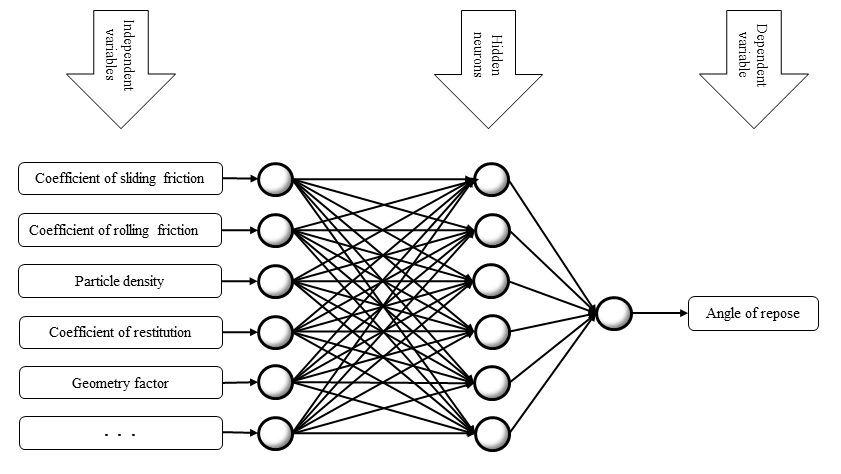
\includegraphics[width=.96\columnwidth]{images/129NN22}
\caption[ANN Scheme]{Artificial Neural Network (\acs{ANN}) Scheme. Regressors
are show in the left-hand side of the image. An example of a response is shown
in the right-hand side of the image.}
\label{fig:018nnscheme}
\end{figure}
\begin{table}[h]
\centering
\begin{tabular}{lcccc}
\hline
 &  \ac{mus} & \ac{mur} & \ac{CoR} & \ac{rhop}  \\
  &	$[-]$  & $[-]$   & $[-]$   & $[kg/m3]$ \\
          \hline
    range & $[0.1 \ldots 1.0]$ & $[0.1 \ldots 1.0]$ & $[0.5 \ldots 0.9]$ &
    $[2000 \ldots 3500]$     \\
    \# rnd & 100   & 100   & 25    & 25    \\

\hline
\end{tabular}
\caption[DEM random input values]{DEM random input values. Within each range \#
random values are chosen.}
\label{tab:12DEMRandominputvalues}
\end{table}